\documentclass[a4paper]{article}

\usepackage[french]{babel}
\usepackage[T1]{fontenc}
\usepackage[utf8]{inputenc}
\usepackage{amsmath}
\usepackage{graphicx}
\usepackage{lmodern}
\usepackage[left=3cm, right=3cm, bottom=4cm, top=4cm]{geometry}
\usepackage{array}
\usepackage{pdfpages}
\usepackage{listings}
\usepackage{algorithm}
\usepackage{algorithmic}
\usepackage{sidecap}
\usepackage{pdflscape}
\usepackage{hyperref}
\usepackage{tipa}
\usepackage{multirow}
\usepackage[gen]{eurosym}
\DeclareUnicodeCharacter{20AC}{\euro{}}

\usepackage{hyperref}
\hypersetup{    
    colorlinks,
    citecolor=black,
    filecolor=black,
    linkcolor=black,
    urlcolor=black
}

\title{Rapport de planification}

\author
{
    Pierre-Marie {\sc Airiau}\\
    Valentin {\sc Esmieu}\\
    Hoel {\sc Kervadec}\\
    Maud {\sc Leray}\\
    Florent {\sc Mallard}\\
    Corentin {\sc Nicole}
}

\date{\today}

\newcommand{\pagevierge}[0]{\newpage\thispagestyle{empty}\null\newpage}
\newcommand{\glasir}[0]{Glasir}
\newcommand{\ttable}[0]{{\sc Table}}
\newcommand{\ffigure}[0]{{\sc Figure}}

\newcommand{\nomRepart}[1]{\multicolumn{2}{c||}{\textbf{#1}}}
\newcommand{\nomRepartt}[1]{\multicolumn{2}{c|}{\textbf{#1}}}

\begin{document}
    % Ouh c'est sale.
    \hypersetup{pageanchor=false}
    
\includepdf[pages=1]{figure/couv.pdf}
    \hypersetup{pageanchor=true}
    
    \newpage
    \thispagestyle{empty}
    \mbox{}
    
    \newpage
    % A decommenter pour la release
    % \setcounter{tocdepth}{2}
    \tableofcontents
    \setlength{\parskip}{10pt}
    
    \newpage
    \thispagestyle{empty}
    \mbox{}

    \newpage
    \section{Introduction}
	La sécurisation des systèmes est une problématique majeure de la société moderne. En ce sens, de nombreuses méthodologies ont été développées~\cite{introSecurite,ADTreeKordy} dans le but d'identifier les risques et de les quantifier. C'est avec cet objectif que le concept d'arbres d'attaque et de défense (ADTrees) a vu le jour.

	Lors de la phase de pré-étude, nous avons pu comprendre l’intérêt pratique de la construction des ADTrees. Leur utilisation permet d'identifier de manière précise les différentes attaques possibles contre un système et de les valuer en termes de coût, de probabilité, etc. ADTool~\cite{adtool_paper} (Attack-Defense Tree Tool), un logiciel libre développé pour l'implémentation de ces arbres sur support informatique, a été mis à disposition pour ce projet. Lors de sa prise en main, des limites ont été constatées. En effet, dans un cas concret d'expertise en sécurité, le système doit faire face à une multitude d'attaques possibles et, par conséquent, l'ADTree qui les modélisera sera de très grande taille. Dans ce cas, il est très difficile pour l'expert d'en extraire des informations pertinentes au premier coup d’œil. Or, ADTool ne fournit pas d'outil permettant à l'utilisateur de simplifier l'analyse de l'arbre. 

	L'objectif de ce projet est donc la création d'un logiciel intégrant ADTool et permettant de faciliter le travail d'un expert en sécurité, en lui fournissant des outils pour analyser facilement ses ADTrees. Ce logiciel portera le nom de \glasir{}  (prononcé [\textipa{glaziK}]). Il s'agit du nom d'un arbre aux feuilles d'or dans la mythologie nordique~\cite{vikingCulture}.

	Ce rapport présente les spécifications fonctionnelles de \glasir{}. Tout d'abord, les limites d'ADTool seront abordées, afin de justifier l'intérêt de \glasir{}. Puis nous détaillerons les différentes fonctionnalités destinées à l'analyse des ADTrees. Enfin, quelques améliorations supplémentaires seront également précisées pour offrir un meilleur confort de création et édition d'arbres. Ces spécifications seront faites en prenant en exemple une situation précise : celle d'un expert en sécurité chargé par le Service des Transports en commun de l'Agglomération Rennaise (STAR) de déterminer les failles de leurs systèmes de paiement.

    \newpage
    %\section{Contexte}
	\label{sec:retrospective}
	
\subsection{Périmètre fonctionnel}

\subsection{Éléments en entrée}

\subsection{Rétrospective}
	\label{sec:retrospective}

	Nous avons déjà rédigé deux rapports dans le cadre de ce projet, nous permettant d'en aborder différents aspects. Leur contenu est brièvement rappelé ci-dessous.

	\paragraph{Rapport de pré-étude} Nous avons commencé ce projet par une étude de l'existant : la théorie des ADTrees ainsi que la découverte d'ADTool, un logiciel permettant d'en créer et d'en manipuler. Nous avons relevé lors de cette étude des lacunes empêchant une analyse poussée des ADTrees. Le contexte (transports en commun, plus particulièrement le STAR) a lui aussi été traité, afin de mieux cerner notre cas d'étude. Il est apparu que les attaques contre les transports en commun sont assez fréquentes, qu'elles soient volontaires ou non. Nous entendons par \og attaque \fg{} tout événement nuisant au bon fonctionnement du réseau de transport. Suite à cela, nous avons été en mesure de proposer un premier cahier des charges. Ce dernier a été étoffé et précisé dans le second rapport.

	\paragraph{Rapport de spécifications fonctionnelles} Les fonctionnalités du logiciel ont été décrites de façon exhaustive. Cela nous a permis de fournir une première ébauche de l'architecture de \glasir{}, comprenant les dépendances entre les modules, et d'établir les différents liens les unissant. Cela nous a donné une vision plus globale et claire du projet, nous permettant de hiérarchiser les tâches à effectuer. Pour finir, nous avons proposé une planification succincte, développée dans le présent rapport. Celle-ci prévoyait la séparation du développement en de nombreuses versions.

	Celles-ci ont évolué depuis, et sont présentées en détail dans la section suivante.
    
    %\section{Méthode de gestion de projet}
	\label{sec:gestion}


Au cours de nos réunions, nous nous sommes naturellement dirigés vers une méthode agile ressemblant à \og Scrum \fg. Nous nous réunissons une fois par semaine afin de discuter de l'avancement de nos tâches respectives et faire part de nos difficultés. Nous définissons en fonction de cela des tâches à effectuer la semaine suivante. 
	Chaque version sera composée de sprints au cours desquels nous nous consacrerons à un sous-ensemble de tâches nécessaires à une version. %whattt ???
	

		
    %\section{Tâches unitaires}
	\label{sec:taches_unitaires}

	Les tests unitaires étants réalisés au fûr et à mesure, ils sont prit en compte dans l'estimation du temps nécessaire à la réalisation des tâches.

	\subsection{Version intermédiaire 1}

		\begin{table}[h]
			\centering
			\begin{tabular}{|c|r|l|c|r|}
				\hline
				\textbf{Cible} & \textbf{Id} & \textbf{Tâche} & \textbf{Technologies} & \textbf{Durée}\\
				\hline

				\multirow{5}{*}{\glasir{}} & 1.1 & Créer squelette interface & WPF & 3h\\
				\cline{2-5}
				 & 1.2 & Gestion des fichiers du projet & C\# & 10h\\
				\cline{2-5}
				 & 1.3 & Intégrer ADTool dans application & JNI & 10h\\
				\cline{2-5}
				 & 1.4 & \'Evaluateur de fonction & Java & 6h\\
				\cline{2-5}
				 & 1.5 & Interface évaluateur & WPF & 4h\\
				\hline

				\multirow{3}{*}{ADTool} & 1.6 & Valuer arbre & \multirow{3}{*}{Java} & 9h\\
				\cline{2-3} \cline{5-5}
				 & 1.7 & Refonte du langage des arbres & & 8h\\
				\cline{2-3} \cline{5-5}
				 & 1.8 & Vue globale des paramètres & & 6h\\
				\hline

				\multicolumn{4}{|l|}{\bf Total} & {\bf 56h}\\
				\hline
			\end{tabular}
			\caption{Tableau tâches version intermédiaire 1}
			\label{fig:taches_units_1}
		\end{table}

	\subsection{Version intermédiaire 2}

		\begin{table}[h]
			\centering
			\begin{tabular}{|c|r|l|c|r|}
				\hline
				\textbf{Cible} & \textbf{Id} & \textbf{Tâche} & \textbf{Technologies} & \textbf{Durée}\\
				\hline

				\multirow{4}{*}{\glasir{}} & 2.1 & Algorithme de filtrage & C++ & 24h\\
				\cline{2-5}
				 & 2.2 & Interface filtre & WPF & 15h\\
				\cline{2-5}
				 & 2.3 & Multiples instances d'ADTool & C++, WPF & 15h\\
				\cline{2-5}
				 & 2.4 & Affichage de l'arbre filtré & C++, WPF & 5h\\
				\hline

				\multirow{1}{*}{ADTool} & 2.5 & Couper/copier/coller & \multirow{1}{*}{Java} & 10h\\
				\hline

				\multicolumn{4}{|l|}{\bf Total} & {\bf 69h}\\
				\hline
			\end{tabular}
			\caption{Tableau tâches version intermédiaire 2}
			\label{fig:taches_units_2}
		\end{table}

	\subsection{Version finale}

		\begin{table}[h]
			\centering
			\begin{tabular}{|c|r|l|c|r|}
				\hline
				\textbf{Cible} & \textbf{Id} & \textbf{Tâche} & \textbf{Technologies} & \textbf{Durée}\\
				\hline

				\multirow{4}{*}{\glasir{}} & 3.1 & Optimiseur & C++, WPF & 15h\\
				\cline{2-5}
				 & 3.2 & Bibliothèque de modèles & C++, WPF & 10h\\
				\cline{2-5}
				 & 3.3 & Harmonisation interface & WPF & 5h\\
				\cline{2-5}
				 & 3.4 & Packaging & ? & 10h\\
				\hline

				\multirow{1}{*}{ADTool} & 3.5 & Ctrl-z & \multirow{1}{*}{Java} & 8h\\
				\hline

				\multicolumn{4}{|l|}{\bf Total} & {\bf 48h}\\
				\hline
			\end{tabular}
			\caption{Tableau tâches version finale}
			\label{fig:taches_units_3}
		\end{table}    
		
    %\section{Organisation}
	\label{sec:livrables}

	Au cours de nos réunions, nous nous sommes naturellement dirigés vers une méthode agile ressemblant à \og Scrum \fg. Nous nous réunissons une fois par semaine afin de discuter de l'avancement de nos tâches respectives et faire part de nos difficultés. Nous définissons en fonction de cela des tâches à effectuer la semaine suivante. Ainsi, nous avons décidé de livrer trois versions de \glasir{}, dont 2 intermédiaires.
	Chaque version sera composée de sprints au cours desquels nous nous consacrerons à une partie des tâches composant une version.
	Nous présentons ci-dessous la répartition des livrables :
	
	\begin{itemize}
		\item{v 0.1} Paramètres de synthèse :
		\begin{itemize}
			\item{sprint 1} Implémenter l'IHM, y intégrer ADTool, créer un projet, l'afficher dans l'arborescence ;
			\item{sprint 2} Évaluer une formule dans ADTool, la propager dans l'arbre, améliorer le codage des arbres ;
			\item{sprint 3} Rendre visibles plusieurs paramètres, communiquer les formules entre ADTool et \glasir{}, documenter le code et tester ;
		\end{itemize}
		\item{v 0.2} filtre :
		\begin{itemize}
			\item{sprint 1} Définir l'algorithme de filtrage, créer l'IHM ;
			\item{sprint 2} Créer un panneau dans \glasir{}, afficher l'arbre résultat, tester ;
			\item{sprint 3} Documenter le code, ouverture simultanée de plusieurs arbres ;
		\end{itemize}
		\item{v 1.0} optimiseur :
		\begin{itemize}
			\item{sprint 1} Implémenter l'algorithme de calcul du chemin optimal, créer le panneau associé dans l'IHM ;
			\item{sprint 2} Annuler une action, créer une bibliothèque de modèles, créer la page HTML ;
			\item{sprint 3} Documenter le code, harmoniser les graphismes.
		\end{itemize}
	\end{itemize}


	Ce plan d'action est amené à changer au fur et à mesure de sa réalisation, ces évolutions étant le but même des méthodes dites \og agiles \fg.
	
	\paragraph{Version intermédiaire 1}


	\paragraph{Version intermédiaire 2}

	\paragraph{Version finale}


    %\section{Risques}
    Nous pouvons d'ores et déjà envisager des situations dans lesquelles nous ne serions pas en mesure de livrer le projet dans l'état que nous avions prévu en ce début d'année scolaire.
    Le facteur principal est bien entendu humain. En effet, la moitié du groupe partant étudier à l'étranger dans le cadre de la mobilité internationale, il se peut que nous ayons légèrement sur-estimé nos capacités de travail et annoncé une tâche trop difficile à exécuter. De plus, sur les trois personnes restant en France, une incapacité à travailler sur le projet, quelle qu'elle soit, aurait des répercussions sur l'avancée globale du livrable. Mais une incapacité de ce type serait accidentelle et très peu probable.
    
    Des problèmes d'ordre technique peuvent également survenir. Il est ainsi possible que nous rencontrions des difficultés à mettre en place la chaîne logicielle prévue, la plupart d'entre nous n'en ayant jamais développé. Nous pourrions ainsi connaître des problèmes dans la communication des différents composants de la chaîne logicielle. Il faudra, pour éviter cela, bien choisir les langages utilisés dans la conception logicielle.
    Une perte de données stockées sur Git, ou bien de fauses manipulations entrainant une perte de données totale ou partielle ralentirait \textit{a minima} le projet, et dans le pire des cas le rendrait impossible à livrer tel que nous l'avons promis. Cependant, Git est équipé d'outils de récupération pour les \textit{commit}, et le projet sera normalement mis à jour (\textit{pull}) sur chacun de nos ordinateurs personnels, réduisant quasimment ce risque à zéro.


    \chapter{Contexte}

	\section{Un contexte mondial}

	Le bon fonctionnement des transports en commun dépend de nombreux facteurs. Qu'il soit humain, ou bien technique, le moindre dysfonctionnement impactera le système entier très rapidement. Ainsi, un simple tour d'horizon de la presse internationale fait vite remonter à la surface de nombreux cas de paralysie des transports publics urbains dans le monde entier.

		\subsection{ Les risques d'atteinte aux passagers }

	Parmi tous les cas de paralysie, les plus marquants à l'échelle internationale sont ceux impliquant des dégâts humains importants parmi les passagers. Il s'agit, dans la plupart des cas, d'attaques terroristes. Bien qu'ils soient relativement rares, le lourd bilan humain de ces attentats marque durablement les esprits.

	C'est le cas de l'attentat à la bombe dans la gare Saint-Michel du train inter-urbain parisien, le 25 juillet 1995, qui provoqua la mort de 8 personnes\cite{stmichel}. L'attaque la plus marquante de l'histoire fut celle du 7 juillet 2005 dans la ville de Londres. Quatre attentats-suicides dans différentes rames de métro provoquent la mort de 56 personnes et en blessent 700 autres. \cite{london_attacks}.

    	\subsection{ Le risque des mouvements sociaux }
    	
	Si ces attaques sont impressionantes et marquantes pour la population, elles restent minoritaires dans les cas de paralysie. Un rapide tour d'horizon de la presse internationale nous montre que la majorité des cas de blocage des transports en communs sont provoqués par le personnel des compagnies gérant ces transports. En effet, lors de conflits sociaux, le personnel possède un énorme moyen de pression sur la hiérarchie car il peut bloquer l'intégralité du traffic en se mettant en grève. 

	C'est le cas à Londres, où un plan de fermeture des guichets du métro a provoqué une grève massive le 28 avril 2014. Cela a entraîné la fermeture des deux tiers des stations et la diminution du traffic de 50\% \cite{tubeApril}. Mais aussi à San Fransisco, en juillet et octobre 2013, où une grève du réseau ferré interurbain (forte de ses 400 000 milles passagers par jour) a paralysé la ville pendant plusieurs jours. \cite{SFbart}

	\section{La situation en France}
	
	En France, il arrive aussi que les réseaux de transports en commun soient mis en difficulté. Les archives ne contiennent pas de traces de graves attentats tels que cités précédemment : la plupart du temps, les troubles sont dûs à des grèves du personnel pouvant refléter différentes réclamations.
	
	\subsection{ Les évènements notables dans tout le pays }

	Commençons par Marseille en décembre 2013, où les conducteurs ont réussi à bloquer la quasi-totalité du réseau pendant plus de deux jours. Ils protestaient contre les salaires, la pénibilité en fin de carrière et la suppression de deux jours de congés. Cela est également arrivé à Lille en mai 2014, où le tramway et les bus ont été immobilisés par les traminots demandant une hausse des salaires.

	Mais parfois, les grèves sont la conséquence de certains incidents survenus lors des trajets. Le plus souvent, il s'agit d'agressions sur le personnel, qui sont plus fréquentes qu'on ne pourrait le penser.

	À Dunkerque en mai 2013 par exemple, un chauffeur subit une agression de la part de voyageurs, qui l'ont poursuivi en voiture jusqu'au terminus de la ligne. Arrivés là, équipés d'extincteurs, ils ont bloqué le bus et menacé ses occupants. La CGT a été avertie, une plainte a été déposée et les conducteurs ont exercé leur droit de retrait, paralysant ainsi le réseau pendant toute une journée.

	C'est ensuite à Douai, en septembre de la même année, que trois contrôleurs sont agressés lors d'un contrôle par une vingtaine de personnes. Des coups sont échangés, les trois hommes finissent à l'hôpital avec des contusions et une entorse au poignet pour l'un d'entre eux. L'ensemble des contrôleurs du réseau exerce alors son droit de retrait, bloquant celui-ci pendant une journée entière.

	Mais qu'en est-il au sein de l'agglomération rennaise, qui nous intéresse tout particulièrement dans le cadre de ce projet ? Commençons par décrire le réseau de transports actuellement en place, ainsi que sa gestion.
		
		\subsection{ Le cas rennais }

	Le réseau de transports rennais est constitué d'une ligne de métro (une deuxième étant en construction) et d'un réseau de bus. Ces deux éléments sont gérés par le STAR (Service des Transports en commun de l'Agglomération Rennaise), qui dépend de la société Keolis Rennes. Le STAR a également mis en place depuis quelques années un système de vélos en libre-service : les vélos STAR. Les usagers peuvent accéder aux différents services du STAR par plusieurs moyens : en achetant des tickets à l'unité (pour bus et métro), ou en utilisant une carte d'abonné rechargeable (la carte Korrigo). 
	
	L'information aux voyageurs passe par 870 écrans dans les bus, 70 dans les stations de métro et 50 bornes d’informations voyageurs (BIV) dans les abribus. Le système d’aide à l’exploitation et à l’information des voyageurs (SAEIV) permet d’indiquer en temps réel le passage du prochain bus, les perturbations, les correspondances, la disponibilité des Vélos STAR… Ces données sont disponibles en open data, et consultables via un service mobile mis à disposition par le STAR.

	Toute cette organisation n'est cependant pas à l'abri des incidents et présente quelques failles : voici un récapitulatif des paralysies les plus importantes que nous avons trouvées.

	En juillet 2009, la ligne de métro a été bloquée pendant près de 20h à la suite d'un violent orage provoquant l'inondation des voies de circulation. Ceci n'est certes pas une attaque volontaire mais cela reste une faiblesse du système qu'il nous a paru intéressant de relever. 

	C'est ensuite en avril 2012 que le réseau STAR entier a été paralysé, en pleine heure de pointe, suite à l'agression d'un chauffeur. À l'époque, la direction recensait 18 agressions depuis le début de l'année, et promettait un redéploiement de ses agents de médiation et de prévention. Une mesure insuffisante pour la CFDT, qui réclamait "une police dédiée aux transports".

	Environ un mois plus tard, en mai, la ligne de métro a été bloquée dès 5h30 du matin. Selon le STAR, il s’agirait d’un problème informatique entre le centre de commandement du métro et les rames : la liaison qui permet de contrôler les rames à distance ne fonctionnait plus. Un service de bus a été mis en place pour limiter les conséquences.

	Ces quelques faits montrent bien l'importance pour le STAR de la mise en place d'un outil d'évaluation des risques, qui comporterait également un répertoire de défenses à utiliser pour contrer ces derniers.

		
		\section{Organisation}
	\label{sec:orga}
	\subsection{La méthode SCRUM}
		\label{subsec:scrum}

	Afin de définir la méthode de gestion de projet à mettre en place pour la réalisation de \glasir{}, nous avons débattu ensemble des différentes méthodes à notre disposition. A la suite de 	nos discussions en réunions, nous nous sommes dirigés vers une méthode agile proche du \og \textsc{scrum} \fg{}. Ce choix s'est fait sur les points qui sont détaillé ci-dessous :

	L'organisation des rôles que nous avons mise en place depuis le début du projet se base sur un rôle de \og Coordinateur \fg{}, qui est responsable de la réalisation et du rendu d'un livrable (rapport, version logicielle, etc). Ce rôle tourne à chaque nouveau livrable, de sorte que chacun des membres de l'équipe l'exerce au moins une fois. Le rôle de coordinateur que nous avons défini nous a donc semblé correspondre au rôle de ScrumMaster tel que défini dans la méthode \textsc{scrum}.

	Le coordinateur endosse également la responsabilité de Product Owner, qu'il partage avec les encadrants du Projet pour ce qui est de la définition des Objectifs et surtout de l'acceptation des livrables.

	En place de la mêlée quotidienne du \textsc{scrum}, nous nous réunissons une fois par semaine afin de discuter de l'avancement de nos tâches respectives et faire part de nos difficultés. Nous avons décidé d'adopter un rythme hebdomadaire plutôt que quotidien car nous ne travaillerons pas à temps plein sur le projet et ce rythme nous a donc semblé plus adéquat. Nous définissons en fonction des retours en réunion les éventuels ajustements à effectuer la semaine suivante et dans le reste de la planification.

	Enfin, chaque version sera composée de sprints au cours desquels nous nous consacrerons à un sous-ensemble de tâches nécessaires à la réalisation d'une version de \glasir{}. Ces tâches constitueront les Users Stories du projet, et sont détaillées dans la \textsc{sous-section}~\ref{subsec:taches_unitaires}.  
	
	\subsection{Tâches unitaires et estimations}
		\label{subsec:taches_unitaires}

	Nous avons décidé de livrer trois versions de \glasir{} : deux intermédiaires et une finale. Ces dernières ont elles-mêmes été divisées en tâches unitaires, décrites dans cette section.
	
	Pour déterminer le temps nécessaire à l'accomplissement de chaque tâche, nous avons combiné les méthodes d’estimation \og Analogique \fg{} et \og Expertise \fg{}. En effet, la méthode \og Analogique \fg{} consiste à estimer la durée d'une tâche par analogie avec une tâche similaire déjà effectuée (au sein d'un autre projet par exemple). La méthode \og Expertise \fg{}, quant à elle, repose sur le jugement d'un expert. Bien qu'aucun membre de notre groupe ne puisse réellement se considérer comme tel, nos stages respectifs ont tout de même permis d'apporter des avis constructifs sur l'estimation de la durée des tâches.
	
	Les résultats de ces différentes estimations sont décrits ci-après pour chaque version. Il est à noter que les tests et la rédaction de la documentation sont pris en compte dans l'estimation du temps nécessaire à la réalisation de chacune des tâches.
	

		\subsubsection{Version 0.1}
			Huit grandes tâches ont été identifiées pour cette version et sont présentées dans la {\sc Table} \ref{tab:taches_units_1}. 
			\begin{table}[H]
				\centering
				\begin{tabular}{|c|r|l|c|r|}
					\hline
					\textbf{Cible} & \textbf{Id} & \textbf{Tâche} & \textbf{Technologies} & \textbf{Durée}\\
					\hline

					\multirow{5}{*}{\glasir{}} & 1.1 & Squelette interface & WPF & 6h\\
					\cline{2-5}
					 & 1.2 & Gestion fichiers projet & C++ & 20h\\
					\cline{2-5}
					 & 1.3 & Intégration ADTool dans \glasir & JNI & 20h\\
					\cline{2-5}
					 & 1.4 & \'Evaluateur de fonction & Java & 12h\\
					\cline{2-5}
					 & 1.5 & Interface évaluateur & WPF & 8h\\
					\hline

					\multirow{3}{*}{ADTool} & 1.6 & Valuation ADTrees & \multirow{3}{*}{Java} & 18h\\
					\cline{2-3} \cline{5-5}
					 & 1.7 & Refonte langage des ADTrees & & 16h\\
					\cline{2-3} \cline{5-5}
					 & 1.8 & Vue globale des paramètres & & 12h\\
					\hline

					\multicolumn{4}{|l|}{\bf Total} & {\bf 112h}\\
					\hline
				\end{tabular}
				\caption{Tâches associées à la version 0.1.}
				\label{tab:taches_units_1}
			\end{table}
			
			
			La réalisation de cette version sera découpée en trois sprints, présentés ci-dessous :

			\noindent\textbf{Sprint 1} Création de l'interface utilisateur de base de \glasir{}, intégration du logiciel ADTool en tant que fenêtre de \glasir{}, possibilité de création d'un nouveau projet et sa sauvegarde, affichage des différents arbres d'un projet dans un dock sous forme d'arborescence.\newline
			\textbf{Sprint 2} Reconnaissance d'une formule mathématique par le logiciel ADTool, création d'un paramètre en fonction de l'évaluation de cette formule, et l'amélioration de la représentation des arbres sous forme d'une grammaire au sein d'ADTool.\newline
			\textbf{Sprint 3} Affichage de plusieurs paramètres par nœud d'un arbre, possibilité de communication entre le module éditeur de fonction de \glasir{} et la partie création d'un paramètre de synthèse implémentée précédemment dans ADTool.\newline


		\subsubsection{Version 0.2}
			Le développement de la version 0.2 est découpé en cinq tâches, visibles dans la {\sc table} \ref{tab:taches_units_2}.
			\begin{table}[h]
				\centering
				\begin{tabular}{|c|r|l|c|r|}
					\hline
					\textbf{Cible} & \textbf{Id} & \textbf{Tâche} & \textbf{Technologies} & \textbf{Durée}\\
					\hline

					\multirow{4}{*}{\glasir{}} & 2.1 & Algorithme filtrage & C++ & 24h\\
					\cline{2-5}
					 & 2.2 & Interface filtre & WPF & 15h\\
					\cline{2-5}
					 & 2.3 & Multiples instances d'ADTool & C++, WPF & 20h\\
					\cline{2-5}
					 & 2.4 & Affichage arbre filtré & Java, WPF & 16h\\
					\hline

					\multirow{1}{*}{ADTool} & 2.5 & Couper/copier/coller & \multirow{1}{*}{Java} & 25h\\
					\hline

					\multicolumn{4}{|l|}{\bf Total} & {\bf 100h}\\
					\hline
				\end{tabular}
				\caption{Tâches associées à la version 0.2.}
				\label{tab:taches_units_2}
			\end{table}
			
			Nous avons réparti les tâches en trois sprints :

			\noindent\textbf{Sprint 4} Implémentation de l'algorithme de filtrage, permettre l'ouverture de plusieurs instances d'ADTool au sein de différents onglets de l'interface de \glasir{}.\newline 
			\textbf{Sprint 5} Affichage du panneau relatif à ce module au sein de l'interface utilisateur de \glasir{}. Implémentation de la fonction couper/copier-coller.\newline % ou durant le snd sprint?
			\textbf{Sprint 6} Affichage de l'arbre filtré.

		\subsubsection{Version 1.0}
			Quatre tâches ont été identifiées pour la version 1.0 de \glasir{}, regroupées dans la {\sc Table} \ref{tab:taches_units_3}.
			\begin{table}[h]
				\centering
				\begin{tabular}{|c|r|l|c|r|}
					\hline
					\textbf{Cible} & \textbf{Id} & \textbf{Tâche} & \textbf{Technologies} & \textbf{Durée}\\
					\hline

					\multirow{4}{*}{\glasir{}} & 3.1 & Optimiseur & C++, WPF & 30h\\
					\cline{2-5}
					 & 3.2 & Bibliothèque de modèles & C++, WPF & 20h\\
					\cline{2-5}
					 & 3.3 & Harmonisation interface & WPF & 16h\\
					\cline{2-5}
					 & 3.4 & Packaging & ? & 8h\\
					\hline

					\multirow{1}{*}{ADTool} & 3.5 & Ctrl-Z & \multirow{1}{*}{Java} & 16h\\
					\hline

					\multicolumn{4}{|l|}{\bf Total} & {\bf 90h}\\
					\hline
				\end{tabular}
				\caption{Tâches associées à la version 1.0.}
				\label{tab:taches_units_3}
			\end{table}
			
			Les sprints se composeront de :

			\noindent\textbf{Sprint 7} Implémentation de l'algorithme de l'optimiseur, création d'une bibliothèque de modèles.\newline
			\textbf{Sprint 8} Affichage du panneau de l'optimiseur dans \glasir{}, possibilité d'annuler une action dans ADTool.\newline
			\textbf{Sprint 9} Harmonisation de l'interface et réalisation du packaging. \newline

		%TODO estimations
	\subsection{Organisation du groupe et répartition des tâches}
		Lors de la phase de développement de \glasir{}, notre groupe de projet sera réduit à trois étudiants : Pierre-Marie {\sc Airiau}, Valentin {\sc Esmieu} et Maud {\sc Leray}. Les trois autres, Florent {\sc Mallard}, Hoel {\sc Kervadec} ainsi que Corentin {\sc Nicole}, partiront en effet étudier à l'étranger.
		
		Nous comptons donc nous répartir les tâches selon trois composantes générales : Maud L. travaillera principalement sur ADTool, Pierre-Marie A. sur les algorithmes et sur l'interfaçage entre ADTool et \glasir{}, et Valentin E. s'orientera sur l'interface utilisateur de \glasir{}. La {\sc Table} \ref{table:repartition} donne la répartition des tâches plus en détails.
			


		\begin{table}[H]
			\centering
			\begin{tabular}{|l|c|r||c|r||c|r|}
				\hline
				\multirow{2}{*}{} & \nomRepart{Pierre-Marie A.} & \nomRepart{Valentin E.} & \nomRepartt{Maud L.}\\
				\cline{2-7}
				 & {\bf Id tâche} & {\bf Durée} & {\bf Id tâche} & {\bf Durée} & {\bf Id tâche} & {\bf Durée}\\
				\hline
				{\bf Version 0.1} & - & {\bf 38h} & - & {\bf 34h} & - & {\bf 40h}\\
				 & 1.3 & 10h & 1.1 & 6h & 1.2 & 10h\\
				 & 1.4 & 12h & 1.2 & 10h & 1.6 & 18h\\
				 & 1.7 & 16h & 1.3 & 10h & 1.8 & 12h\\
				 & - & - & 1.5 & 8h & - & -\\
				\hline
				{\bf Version 0.2} & - & {\bf 39h} & - & {\bf 33h} & - & {\bf 28h}\\
				 & 2.1 & 24h & 2.3 & 20h & 2.4 & 16h\\
				 & 2.2 & 15h & 2.5 & 13h & 2.5 & 12h\\
				\hline
				{\bf Version 1.0} & - & {\bf 25h} & - & {\bf 23h} & - & {\bf 42h}\\
				 & 3.1 & 15h & 3.1 & 15h & 3.2 & 10h\\
				 & 3.2 & 10h & 3.4 & 8h & 3.3 & 16h\\
				 & - & - & - & - & 3.5 & 16h\\
				\hline
				{\bf Total} & \multicolumn{2}{r||}{{\bf 102h}} & \multicolumn{2}{r||}{{\bf 100h}} & \multicolumn{2}{r|}{{\bf 110h}}\\
				\hline
			\end{tabular}
			\caption{Répartition des tâches, par personne et par version.}
			\label{table:repartition}
			\label{tab:repartition}
		\end{table}


	\subsection{Risques}
		\label{subsec:risques}

	%L'implémentation d'un logiciel comporte toujours des risques. Afin de ne pas nous laisser surprendre par ces derniers, nous avons cherché à lister ceux qui nous venaient à l'esprit.

    % Pour que notre projet se déroule le mieux possible, nous avons listé certains événements susceptibles de nous faire prendre du retard. Ils sont répertoriés dans le tableau\ref{fig:risques}, avec les tâches qu'ils concernent. Nous leur avons ajouté les notions de probabilité (Pr) et de criticité (Cr), sur une échelle de 1 à 3 : 1 pour faible, 2 pour moyenne, 3 pour élevée. Enfin, la dernière colonne cite des solutions possibles pour contre les risques énoncés.

    Dans le but de délivrer ce projet dans les délais, une évaluation des risques a été effectuée. Celle-ci a pour but d'identifier les différents facteurs qui pourraient engendrer des difficultés dans la réalisation des tâches et entraîner ainsi un retard, ou une incapacité à implémenter une partie du cahier des charges. Nous avons associé à chaque élément de cette liste les notions de probabilité (Pr) et de criticité (Cr), sur une échelle de 1 à 3 : 1 pour faible, 2 pour moyenne, 3 pour élevée. Dans le but de réagir au mieux en cas d’apparition de ces aléas, des solutions ont été définies. Le résultat de cette réflexion est présenté dans la \textsc{table}~\ref{fig:risques}. 


	\begin{table}[H]
		\centering
		\begin{tabular}{|p{4cm}|l|l|l|p{4cm}|}
		\hline
            \textbf{Risque} & \textbf{Tâches concernées} & \textbf{Pr.} & \textbf{Cr.} & \textbf{Solution}\\
            \hline
            Mauvaise estimation des durées nécessaires aux tâches unitaires & 
                Toutes & 3 & 3 &
                Bien s'organiser et respecter les délais\\ 
            \hline
            Apparition d'un bug difficile à corriger & 
                Toutes & 3 & 3 &
                Faire des tests unitaires\\
            \hline
            Difficulté à créer une grammaire & 
                1.4 & 1 & 2 &
                Simplifier les expressions à évaluer\\ 
            \hline
            Manque de connaissances techniques & 
                Toutes & 3 & 3 &
                Approfondir nos connaissances\\ 
            \hline
            Rédaction trop tardive de la documentation & 
                Toutes & 2 & 1 &
                Commenter le code au fur et à mesure\\
            \hline
            Mauvaise compréhension du code d'ADTool & 
                Toutes celles sur ADTool & 2 & 2 &
                Contacter le développeur d'ADTool\\ 
            \hline
            Mauvaise communication entre ADTool et \glasir{} & 
                1.4, 2.1, 3.1 & 2 & 3 &
                Utiliser le fichier XML lisible par ADTool\\ 
            \hline
            Perte de temps sur une tâche secondaire & 
                Toutes & 2 & 1 &
                Compter ses heures, faire le point lors des réunions\\ 
            \hline
            Algorithme ralentissant le logiciel & 
                3.1, 2.2 & 1 & 1 &
                Optimiser l’algorithme\\ 
            \hline
            Échec de l'intégration d'ADTool dans \glasir{} & 
                1.2 & 1 & 3 &
                Lancer ADTool séparément\\ 
            \hline
		\end{tabular}
		\caption{Tableau des risques}
		\label{fig:risques}
	\end{table}
	

    \section{Séquencement}
	\label{sec:sequencement}
	Pour établir notre planification, nous avons utilisé le logiciel MS Project. Les diagrammes ci-dessous tiennent compte des différents jalons qui ont été posés, soit imposés à tous dans les projets de 4INFO, soit définis nous-même.

	\subsection{Diagramme de Gantt}
		Le diagramme de Gantt visible sur la \ffigure{} \ref{fig:gantt} illustre le séquencement de notre projet. Les tâches ont été attribuées à une personne, et les durées ont été calculées pour une moyenne d'une heure-et-demi de travail personnel par jour. Les semaines du 18 et 25 mai, bloquées pour les 4INFO, la durée du travail personnel a été porté à 4h par jour. 

	\subsection{Répartition de la charge de travail}
		Le planning de la \ffigure{} \ref{fig:planning_charge} illustre le cumul des heures de travail pour chaque personne. Nous avons essayé d'être homogènes dans la répartition des tâches de chacun.

		\begin{landscape}
		 	\begin{figure}
	            \centering
	            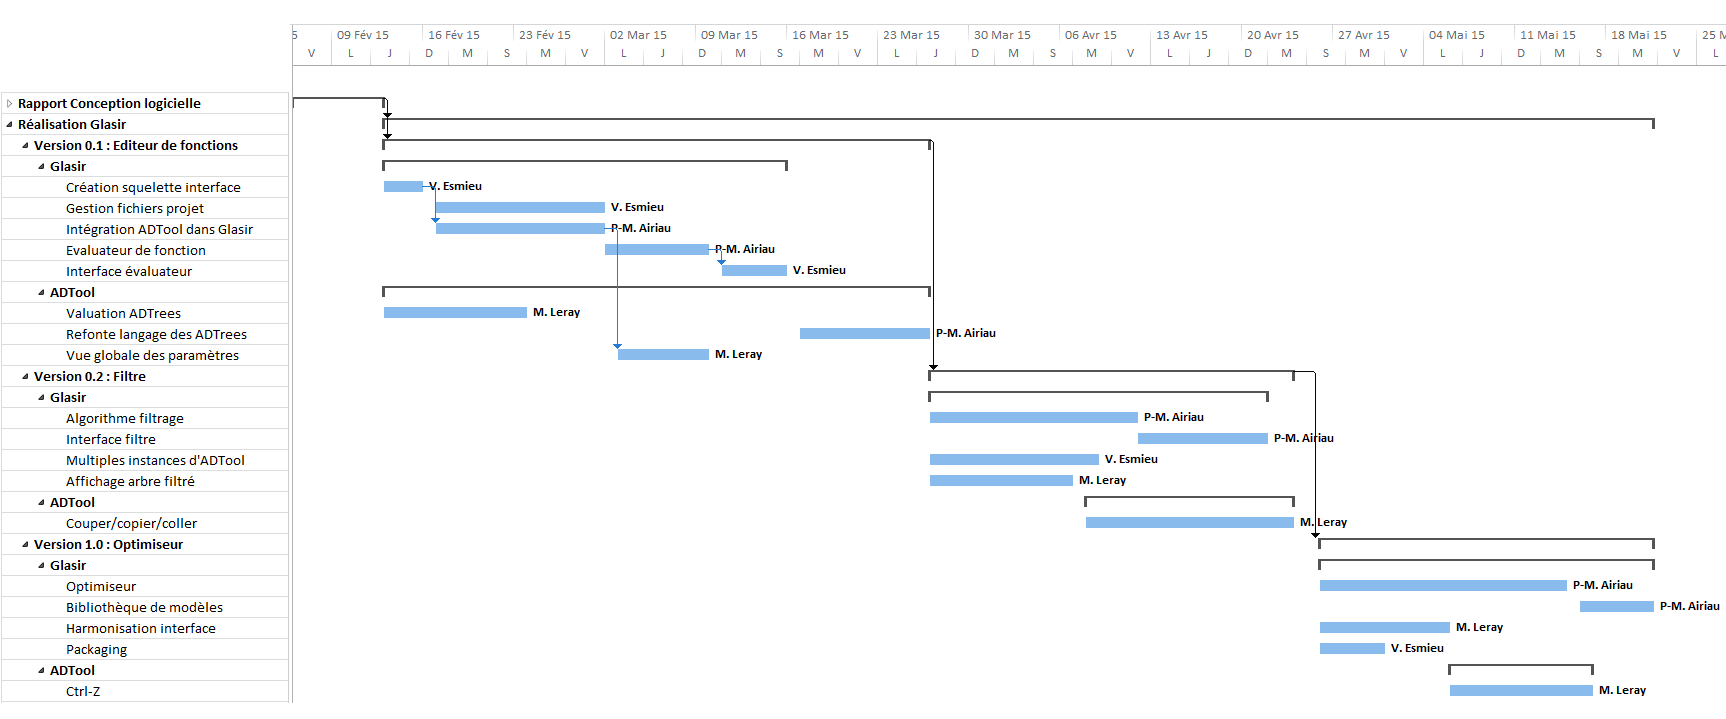
\includegraphics[height=0.70\textwidth]{figure/DiagGantt.png}
	            \caption{Diagramme de Gantt présentant la chronologie des tâches.}
	            \label{fig:gantt}
	        \end{figure}
	    \end{landscape}

		\begin{landscape}
		 	\begin{figure}
	            \centering
	            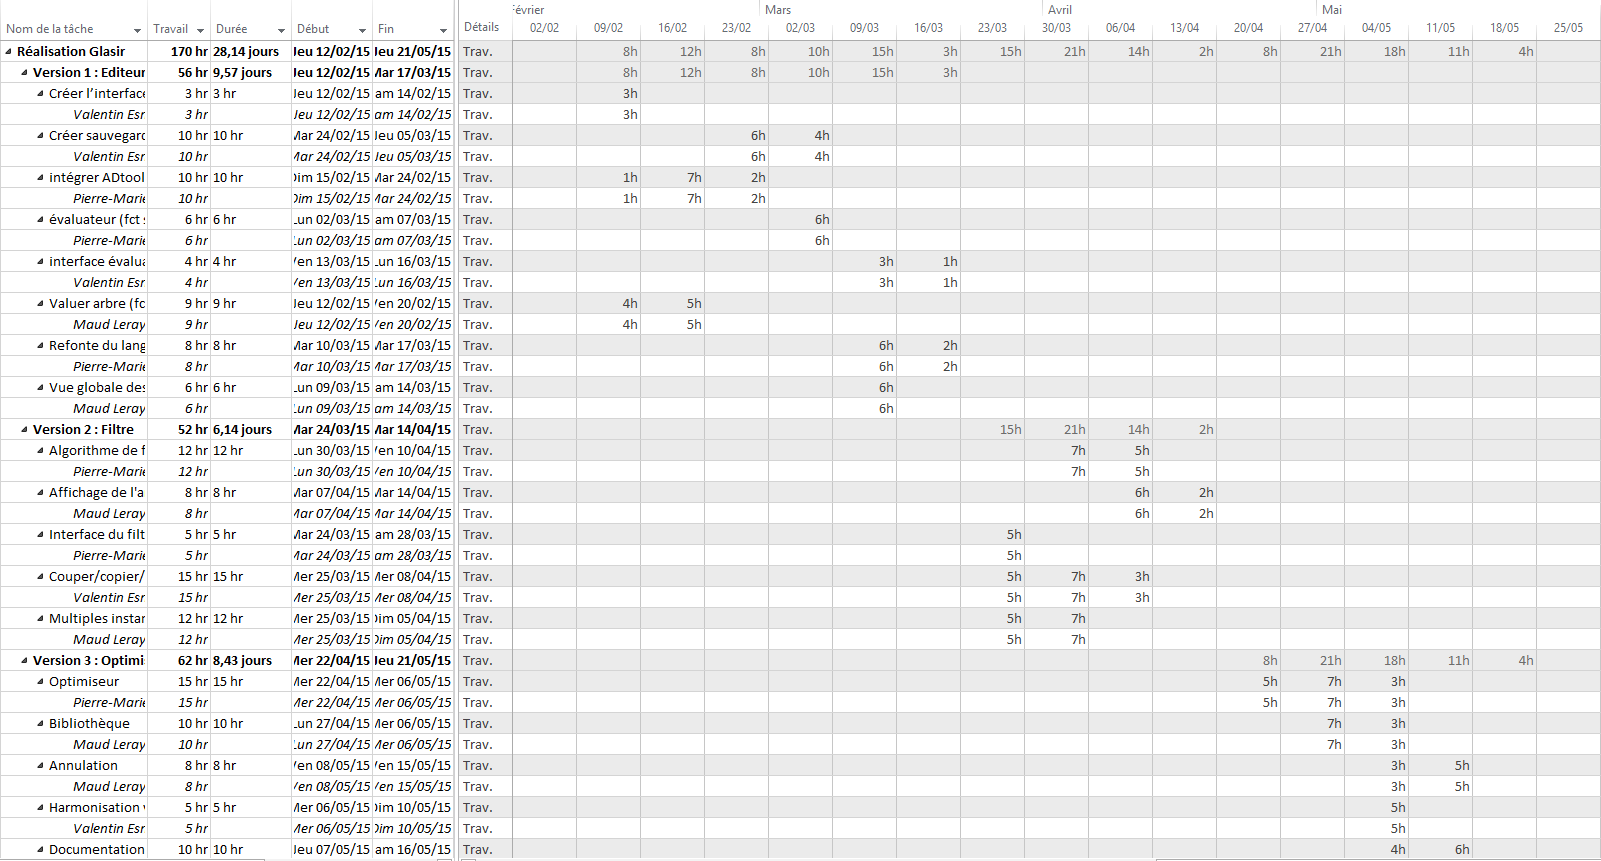
\includegraphics[height=0.70\textwidth]{figure/RepartitionTaches2.png}
	            \caption{Planning des charges réparties par personne}
	            \label{fig:planning_charge}
	        \end{figure}
	    \end{landscape}

	    \subsection{Utilisation des ressources}

    \section{Conclusion}

    %\bibliographystyle{plain}
    %\bibliography{input/biblio}

    % Manoucherie incoming
    \pagevierge
    \ifthenelse{\isodd{\thepage}}
    {\pagevierge}
    {}
    
\includepdf[pages=2]{figure/couv.pdf}
\end{document}